\chapter{Results}\label{chp:results}

\chapterquote{It’s hardware that makes a machine fast. It’s software
  that makes a fast machine slow.}{Craig Bruce}

% Tabels of nodes and triangled visited. Perhaps some statistics over
% wasted iterations by threads waiting for other threads in the warp
% to finish. The high triangle count pr leaf optimization may be
% related to this and makes using highly optimized splitting plane
% calculations in the lower nodes useless.


% Test scenes: Cornell, reflecting dragon2 and sponza

\begin{figure}
  \centering
  \subfloat[The Cornell Box - 36 Triangles.]{
    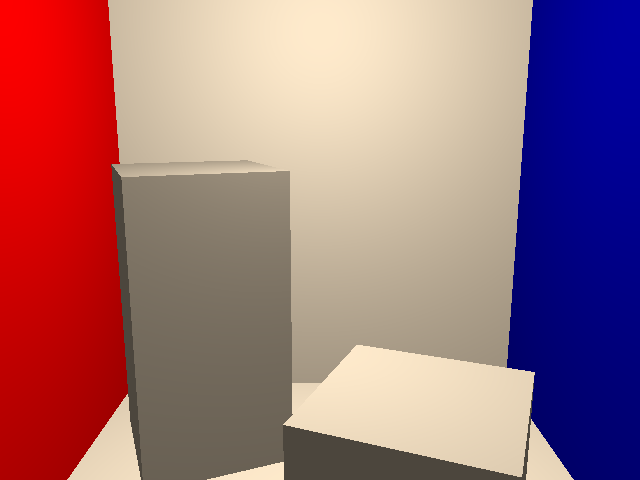
\includegraphics[width=0.3\textwidth]{cornellBox}
  }
  \subfloat[The Reflecting Stanford Dragon - 203k Triangles.]{
    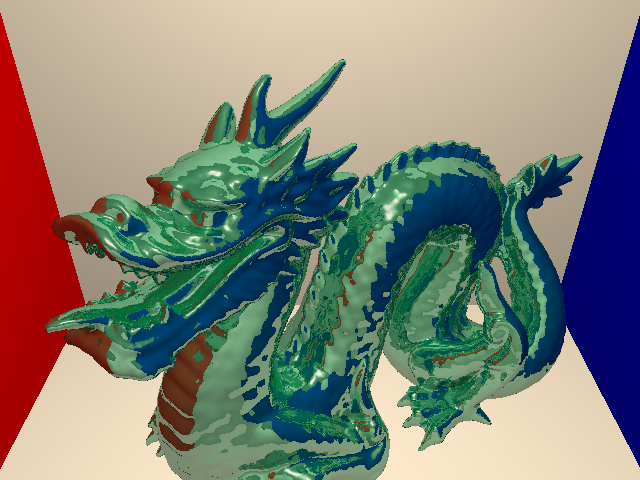
\includegraphics[width=0.3\textwidth]{semiReflectingDragon}
  }
  \subfloat[Sponza - 279k Triangles.]{
    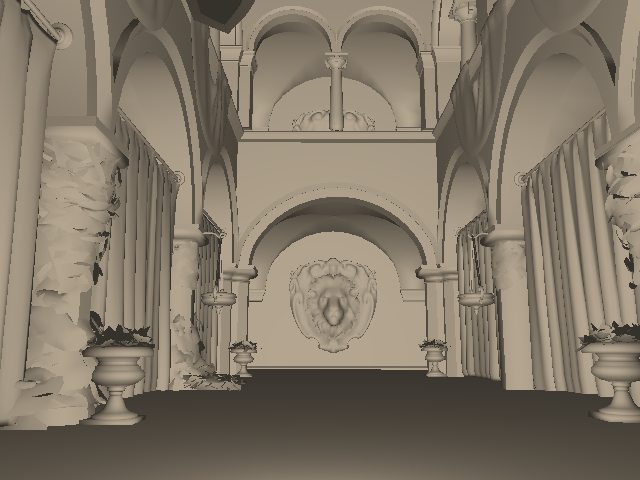
\includegraphics[width=0.3\textwidth]{sponza}
  }
  \caption[Test scenes.]{The 3 test scenes.}
  \label{fig:testScenes}
\end{figure}

% Evaluate ray tracers

% First establish which ray tracer works the best

\begin{figure}
  \centering
  \SetTabelTextSize
  \begin{tabular} {r | c | c | c || c || c || c ||}
    \tabelParam{c}{\textit{Ray} \\ \textit{Tracer:}} &
    \tabelParam{c}{\textit{Ray/triangle}\\\textit{intersection:}} &
    \tabelParam{c}{\textit{Packets:}} &
    \tabelParam{c}{\textit{Leaf} \\ \textit{skipping:}} &
    \tabelScene{Cornell \\Box} & 
    \tabelScene{Reflecting \\Dragon} & 
    \tabelScene{Sponza}\\
      \hline
      \multirow{4}{*}{Exhaustive} & \multirow{2}{*}{Moeller} & No & N/A & 6 \\
      \cline{3-7}
      & & Yes & N/A & 6 \\
      \cline{2-7}
      & \multirow{2}{*}{Woop} & No & N/A & 6 \\
      \cline{3-7}
      & & Yes & N/A & 6 \\
      \hline

  % KD-Restart
  \multirow{8}{*}{KD-Restart} & \multirow{4}{*}{Moeller} & \multirow{2}{*}{No} & No & 6 \\
  \cline{4-7}
  & & & Yes & 6 \\
  \cline{3-7}
  & & \multirow{2}{*}{Yes} & No & 6 \\
  \cline{4-7}
  & & & Yes & 6 \\
  \cline{2-7}
  & \multirow{4}{*}{Woop} & \multirow{2}{*}{No} & No & 6 \\
  \cline{4-7}
  & & & Yes & 6 \\
  \cline{3-7}
  & & \multirow{2}{*}{Yes} & No & 6 \\
  \cline{4-7}
  & & & Yes & 6 \\
  \hline

  % Short-Stack
  \multirow{8}{*}{Short-Stack} & \multirow{4}{*}{Moeller} & \multirow{2}{*}{No} & No & 6 \\
  \cline{4-7}
  & & & Yes & 6 \\
  \cline{3-7}
  & & \multirow{2}{*}{Yes} & No & 6 \\
  \cline{4-7}
  & & & Yes & 6 \\
  \cline{2-7}
  & \multirow{4}{*}{Woop} & \multirow{2}{*}{No} & No & 6 \\
  \cline{4-7}
  & & & Yes & 6 \\
  \cline{3-7}
  & & \multirow{2}{*}{Yes} & No & 6 \\
  \cline{4-7}
  & & & Yes & 6 \\
  \hline
\end{tabular}
\caption[Stuff]{more stuff}
\label{fig:rayTracerEvaluation}
\end{figure}



% Upper tree creation parameters

% Not creating lower nodes (using None)

\begin{figure}
  \centering
  \SetTabelTextSize
  \begin{tabular} {c | c | c || c || c || c ||}
    % Titel bar: Association scheme | empty space maximization | threshold |
    % Cornell | dragon | sponza
    \multicolumn{1}{c}{\begin{tabular}{c}\textit{Association} \\ \textit{scheme:}\end{tabular}} &
    \multicolumn{1}{c}{\begin{tabular}{c}\textit{Empty Space} \\ \textit{Maximization:}\end{tabular}} &
    \begin{tabular}{c}\textit{Empty Space} \\ \textit{Threshold:}\end{tabular} &
    \tabelScene{Cornell \\ Box} & 
    \tabelScene{Reflecting \\ Dragon} &
    \tabelScene{Sponza}\\
    \hline % Titel end
    \multirow{4}{*}{Dividing} & No & N/A & 1-3 (3)\\
    \cline{2-6}
    & \multirow{3}{*}{Yes} & 15 & \\
    \cline{3-6}
    & & 25 & \\
    \cline{3-6}
    & & 35 & \\
    \hline
    \multirow{4}{*}{Box Inclusion} & No & N/A & \\
    \cline{2-6}
    & \multirow{3}{*}{Yes} & 15 & \\
    \cline{3-6}
    & & 25 & \\
    \cline{3-6}
    & & 35 & \\
    \hline
  \end{tabular}
  \caption[Upper tree creation results.]{Upper tree creation results. --What is
    seen and what parameters where used--}
  \label{fig:upperResults}
\end{figure}


% Lower node creation

\begin{figure}
  \centering
  \SetTabelTextSize
  \begin{tabular}{c |c | c || c || c || c ||}
    \tabelParam{c}{\textit{Bit Mask:}} &
    \tabelParam{c}{\textit{Splitting} \\ \textit{Scheme:}} &
    \tabelParam{c||}{$C_{N}:$} &
    \tabelScene{Cornell \\ Box} & 
    \tabelScene{Reflecting \\ Dragon} &
    \tabelScene{Sponza}\\
    \hline % Titel end
    \multirow{7}{*}{32bit} & None & N/A & \\
    \cline{2-6}
    & \multirow{3}{*}{SAH} & 24 & \\
    \cline{3-6}
    & & 16 & \\
    \cline{3-6}
    & & 8 & \\
    \cline{2-6}
    & \multirow{3}{*}{SSAH} & 24 & \\
    \cline{3-6}
    & & 16 & \\
    \cline{3-6}
    & & 8 & \\
    \hline
    \multirow{7}{*}{64bit} & None & N/A & \\
    \cline{2-6}
    & \multirow{3}{*}{SAH} & 24 & \\
    \cline{3-6}
    & & 16 & \\
    \cline{3-6}
    & & 8 & \\
    \cline{2-6}
    & \multirow{3}{*}{SSAH} & 24 & \\
    \cline{3-6}
    & & 16 & \\
    \cline{3-6}
    & & 8 & \\
    \hline
  \end{tabular}
\end{figure}

% Splitting Schemes:

% Profile the time it takes to create the different trees, especially
% the splitting kernels.

% Compare amount of nodes.

% Tree traversal time.

% Warp coherence: balance between traversal steps and intersections =
% high amount of nodes in the leafs ie even less important to spend
% alot of time on that last split.


\chapter{Conclusion}

\chapterquote{The best thing about a boolean is even if you are wrong,
  you are only off by a bit.}{Anonymous}

\fixme{Conclusion must mirror the goals in chp 1! Do it!}

\chapter{Future Work}\label{chp:future}

\chapterquote{Software is like entropy: It is difficult to grasp,
  weighs nothing, and obeys the Second Law of Thermodynamics; i.e., it
  always increases.}{Norman Augustine}

KD/BVH combination trees: still only carry information for one
dimension, but also provide near and far planes, useful for estimating
the advancement of the ray's $t_{min}$.

Look at stackless raytracers with ropes.

Aila et al.\citebook{Aila2009} has looked at persistent threads to
accelerate raytracing. This could be utilized to accelerate the SAH
calculations of individial nodes.

Optimize triangle divide by excluding uninteresting test cases.
